%--------------------------------------------
%	PACKAGES AND DOCUMENT CONFIGURATIONS
%--------------------------------------------

\documentclass[11pt]{article}
\usepackage{fancyhdr}
\usepackage{pgfplots}
\usepackage{gensymb}
\usepackage[ampersand]{easylist}
\usepackage[a4paper, total={8.5in, 11in}, margin = 1in]{geometry}

\usepackage[version=3]{mhchem} % Package for chemical equations
\usepackage{siunitx} % The \SI{}{} and \si{} command for SI units
\usepackage{graphicx, epstopdf} % Required for the inclusion of images
\usepackage{natbib} % Required to change bibliography style to APA
\usepackage{amsmath} % Required for some math elements
\usepackage[framed,numbered]{matlab-prettifier}
\usepackage{float}
\usepackage{multirow}
\usepackage{listings}
\usepackage{setspace}
\doublespacing

\setlength\parindent{0pt} % Removes all indentation from paragraphs

\renewcommand{\labelenumi}{\alph{enumi}.} % Make numbering in the enumerate environment by letter rather than number 

\setcitestyle{square}

%----------------------------------------------
%	DOCUMENT INFORMATION
%----------------------------------------------
\title{Segmenting Clinton and Obama Voters\\ \vspace{1.0cm}
Assignment 1 \\
\\ \vspace{1.0cm}
Name: Whitney Chu\\
}

   
\date{Date: Wednesday, October 28th, 2020}

\newpage

\begin{document}

\begin{titlepage}
    \centering
    \maketitle
    \thispagestyle{empty}
\end{titlepage}

\pagebreak

\newpage
\thispagestyle{empty}
\textbf{Executive Summary}
\\\\
This case analyzes Hilary Clintons and Barrack Obamas speeches to determine if they were targeting the right voters in the 2008 election. Hilary Clinton’s speech made a rhetorical reference about her understanding the toughness of working night shifts representing the late nights she worked as a lawyer, first lady and senator. Her target audience was middle-class, blue-collar American citizens. Barrack Obama’s speech references how farmers were not receiving any benefit even though produce in grocery stores were increasing in price. From his speech, it seems as if he is targeting farmers and people that work on farms. It is difficult to determine his exact target audience, but there is an underlying meaning that he believes in fairness and equality. The election dataset containing county, votes, and demographics will be analyzed to determine whether Clinton and Obama were targeting the right voters.



\newpage
\thispagestyle{empty}
\tableofcontents
\newpage


\newpage
\pagenumbering{arabic}
\doublespacing



\section{Definition of the Problem}
Hilary Clinton and Barrack Obama both took different campaign approaches and strategies with the goal of winning the election. They both decided to target specific audiences in hopes to win more votes. Clinton presented a “Night Shift” speech, while Obama presented a “Down on the farm speech”. The objective is to determine whether their campaign approaches were effective and to determine if they targeted the right voters. This will be accomplished by analyzing and comparing the election dataset consisting of different demographics against the number of votes.  \\


\section{Description of Data}
The dataset contains a lot of information on county, the number of votes and demographics. County include the state, region, land area, election date and election type. The votes include the number of votes for each person, as well as the total number of votes.  The largest section is demographics as that is the information regarding the voters and allow Clinton and Obama to effectively target specific audiences. The demographics include, age, race, education level, income, employment, language spoken, medical care programs, social security programs, disabilities, housing, population and farm area.

\section{Preparation of Data}
Tableau and R Studio were used to analyze the data. The R code provided was significantly adjusted to provide a good insight on the problem at hand and tableau was used to visualize the data and trends in the data. Tableau displayed the relationships between the votes, states and demographics. Correlation plots were created in R Studio to analyze the relationship of votes to the other variables to find the significant predictors. In order to better compare the data, for both candidates, margin, margin percent and wins were taken into account. The margin was calculated by subtracting one candidates votes by the other candidates votes. The margin percent was calculated by dividing the margin by total votes for the candidate. The wins per candidate compares whether the margin is greater than 0, indicating a win. 

\section{Analysis and Results}
The analysis was performed based on the results in R Studio and Tableau. All the relating R code and figures can be found in the Appendix. A simple overview and analysis of the data was performed by looking at the tableau results in appendix A.4. From Figure 11 in the appendix, it is evident that Obama was in the lead with the most votes. The analysis for number of votes compared to the states and regions show that both Clinton and Obama had majority of their votes come from California as seen in in Figure 12,13 and 14. For the months of January and February, both Clinton and Obama had the same trend in the number of votes received per day as seen in  Figure 15. When analyzing the voters per age group, the majority of votes came from citizens below the age of 35 and the least number of votes came from citizens age 65 and above as seen in Figure 16. The overall race distribution in the United States can be seen in Figure 17 and it is evident that the dominant race in the United States is White and the second dominant race is Black. In all four regions, majority of citizens only have a highschool degree and very few citizens also obtain a bachelors degree and this is shown in Figure 18. The unemployment rate in the US is fairly  low and there is a large number of retired citizens that used to work. This distribution can be found in Figure 19. Figure 20 displays the income per region by comparing the amount of voters than have an income over 75k and those living in poverty. In there Midwest, northeast and West regions, there are more people with an income over 75k, however the south region has more people living in poverty. \\

Correlation plots for Clinton and Obama in the appendix (A.2 and A.3) show which variables are correlated with margin, margin percent and wins and the audience they should target. For Clinton, the following variables are correlated: state, FIPS, unemployment rate, poverty, Hispanic, americanindian, white, age65andabove, electiontype, diabilities, retiredworkers, socialsecurityrate, socialsecuirty, medicarerate, medicare, speakingnonenglish, samehouse1995and2000, homeowner, and disabilitiesrate. For Obama, the following variables are correlated: region, agebelow35, black, highschool, bachelors, incomeabove75, medianincome, averageincome. All the other variable that were not mentionned did not have any correlation. Clintons target audience was blue-collar, median income citizens and she definitely targeted the right audience. She had a correlation with unemployment rate and retired workers, which shows that she relates to those who are hard workers and at times people may be unemployed looking for jobs and she understands their difficulties. I think she relates well to those that have tough jobs like in construction for example and she could win the votes of those people. There are a lot of blue-collar jobs in the US and a lot of retired workers could have potentially worked for those blue-collar jobs, allowing them to relate to Clinton.Many of the citizens in the United States only have a highschool diploma and with only a highschool diploma, you can only get blue-collar jobs. This is a large majority of the population meaning Clinton could win over a lot of votes for people that can relate. With respect to median income, Obama had a correlation to those citizens, but overall I think Clintons strategy targeted the right audience in order to increase her votes. Theoretically it was a good idea for Obama to target farmers as there are a lot of farmers in the US, however based on the correlation plots, Obama had no correlation to farm area. There is insufficient evidence to conclude that Obama targeted the right voters, although he was in the lead with the most votes. If people read between the lines, Obama’s underlying message in treating people fairly may have been the reason for him winning a lot of votes. I think his intention of targeting farmers was not a good strategy, but there must have been other factors that made more people vote for him. 


\section{Conclusion}
Overall It is very difficult to predict who citizens will vote for as there are many factors taken into consideration when people make this decision and each person has their own thoughts and opinions. Speeches can have a large impact on a voters decision, but people may already have preconceived thoughts. This was only one of the speeches from Clinton and Obama and I’m sure they had other speeches in their campaign that swayed peoples votes. However, from these specific speeches, it is evident that Clintons speech did in fact attract blue-collar individuals as she related to many of the citizens jobs, but there was not enough evidence that Obama targeted the right audience. Clinton should continue this strategy or even target other demographics such as age65andabove that had a correlation and Obama should target other demographics like black and highschool which have a correlation. In retrospect, although Obama’s speech did not target the right voters, he was still able to convince citizens to vote for him, dominating the number of votes. Many factors were not considered and this was only one speech at the beginning of the campaign, so it is difficult to predict the future POTUS from this data. 



\newpage
\pagenumbering{arabic}% resets `page` counter to 1
\renewcommand*{\thepage}{A\arabic{page}}
\appendix 

\section{Appendix}
\lstset{language=R,
    basicstyle=\small\ttfamily,
    stringstyle=\color{DarkGreen},
    otherkeywords={0,1,2,3,4,5,6,7,8,9},
    morekeywords={TRUE,FALSE},
    deletekeywords={data,frame,length,as,character},
    keywordstyle=\color{blue},
    commentstyle=\color{DarkGreen},
    breaklines=true
}
\subsection{Preview and Preparation of the data in R Studio}
\subsubsection{R Code to preview features of the dataset}
\begin{lstlisting}[language=R]
summary(election_data)
election_data <- as.data.frame(election_data)
str(election_data)
nrow(election_data)
election_data
dim(election_data)
\end{lstlisting}

\subsubsection{R Code to convert categorical variables to a factor data type}
\begin{lstlisting}[language=R]
election_data$Region <- as.factor(election_data$Region)
election_data$Region <- as.numeric(c("1", "2", "3", "4"))
election_data$County <- as.factor(election_data$County)
election_data$State <- as.factor(election_data$State)
election_data$ElectionType <- as.factor(election_data$ElectionType)
election_data$Region <- as.factor(election_data$Region)
str(election_data)
dim(election_data)
\end{lstlisting}

\subsubsection{R Code to check for missing/NA values}
\begin{lstlisting}[language=R]
colSums(is.na(election_data))
\end{lstlisting}

\subsubsection{R Code to replace missing/NA values with the mean}
\begin{lstlisting}[language=R]
election_data
election_data$TotalVote <- ifelse(is.na(election_data$TotalVote), mean(election_data$TotalVote, na.rm=TRUE), election_data$TotalVote)
election_data$Clinton <- ifelse(is.na(election_data$Clinton), mean(election_data$Clinton, na.rm=TRUE), election_data$Clinton)
election_data$Obama <- ifelse(is.na(election_data$Obama), mean(election_data$Obama, na.rm=TRUE), election_data$Obama)
election_data$Black <- ifelse(is.na(election_data$Black), mean(election_data$Black, na.rm=TRUE), election_data$Black)
election_data$Asian <- ifelse(is.na(election_data$Asian), mean(election_data$Asian, na.rm=TRUE), election_data$Asian)
election_data$AmericanIndian <- ifelse(is.na(election_data$AmericanIndian), mean(election_data$AmericanIndian, na.rm=TRUE), election_data$AmericanIndian)
election_data$HighSchool <- ifelse(is.na(election_data$HighSchool), mean(election_data$HighSchool, na.rm=TRUE), election_data$HighSchool)
election_data$Bachelors <- ifelse(is.na(election_data$Bachelors), mean(election_data$Bachelors, na.rm=TRUE), election_data$Bachelors)
election_data$Poverty <- ifelse(is.na(election_data$Poverty), mean(election_data$Poverty, na.rm=TRUE), election_data$Poverty)
election_data$IncomeAbove75K <- ifelse(is.na(election_data$IncomeAbove75K), mean(election_data$IncomeAbove75K, na.rm=TRUE), election_data$IncomeAbove75K)
election_data$MedianIncome <- ifelse(is.na(election_data$MedianIncome), mean(election_data$MedianIncome, na.rm=TRUE), election_data$MedianIncome)
election_data$AverageIncome <- ifelse(is.na(election_data$AverageIncome), mean(election_data$AverageIncome, na.rm=TRUE), election_data$AverageIncome)
election_data$UnemployRate <- ifelse(is.na(election_data$UnemployRate), mean(election_data$UnemployRate, na.rm=TRUE), election_data$UnemployRate)
election_data$SpeakingNonEnglish<- ifelse(is.na(election_data$SpeakingNonEnglish), mean(election_data$SpeakingNonEnglish, na.rm=TRUE), election_data$SpeakingNonEnglish)
election_data$Medicare <- ifelse(is.na(election_data$Medicare), mean(election_data$Medicare, na.rm=TRUE), election_data$Medicare)
election_data$MedicareRate <- ifelse(is.na(election_data$MedicareRate), mean(election_data$MedicareRate, na.rm=TRUE), election_data$MedicareRate)
election_data$SocialSecurity <- ifelse(is.na(election_data$SocialSecurity), mean(election_data$SocialSecurity, na.rm=TRUE), election_data$SocialSecurity)
election_data$SocialSecurityRate <- ifelse(is.na(election_data$SocialSecurityRate), mean(election_data$SocialSecurityRate, na.rm=TRUE), election_data$SocialSecurityRate)
election_data$RetiredWorkers <- ifelse(is.na(election_data$RetiredWorkers), mean(election_data$RetiredWorkers, na.rm=TRUE), election_data$RetiredWorkers)
election_data$Disabilities <- ifelse(is.na(election_data$Disabilities), mean(election_data$Disabilities, na.rm=TRUE), election_data$Disabilities)
election_data$DisabilitiesRate<- ifelse(is.na(election_data$DisabilitiesRate), mean(election_data$DisabilitiesRate, na.rm=TRUE), election_data$DisabilitiesRate)
election_data$Homeowner <- ifelse(is.na(election_data$Homeowner), mean(election_data$Homeowner, na.rm=TRUE), election_data$Homeowner)
election_data$SameHouse1995and2000<- ifelse(is.na(election_data$SameHouse1995and2000), mean(election_data$SameHouse1995and2000, na.rm=TRUE), election_data$SameHouse1995and2000)
election_data$LandArea <- ifelse(is.na(election_data$LandArea), mean(election_data$LandArea, na.rm=TRUE), election_data$LandArea)
election_data$FarmArea <- ifelse(is.na(election_data$FarmArea), mean(election_data$FarmArea, na.rm=TRUE), election_data$FarmArea)

colSums(is.na(election_data))
\end{lstlisting}


\subsubsection{R Code to create a train and test set}
\begin{lstlisting}[language=R]
election_data
election_data_train <- election_data[election_data$ElectionDate < as.Date("2/19/08", format="%m/%d/%y"),]
election_data_train
election_data_test <- election_data[election_data$ElectionDate >= as.Date("2/19/2008", format="%m/%d/%Y"),]
election_data_test
\end{lstlisting}

\subsubsection{R Code for the creation of independent variables for Clinton}
\begin{lstlisting}[language=R]
str(election_data_train)
clinton.data <- as.data.frame(election_data_train[,1:41])
clinton.data
clinton.data$clinton_margin <- ifelse((clinton.data$Clinton - clinton.data$Obama)>0,1,0)
clinton.data$clinton_margin_percent <- ifelse((clinton.data$clinton_margin/clinton.data$TotalVote)>0,1,0)
clinton.data$clinton_wins <- ifelse(clinton.data$clinton_margin >0, 1,0)
names(clinton.data)
\end{lstlisting}

\subsubsection{R Code for the creation of independent variables for Obama}
\begin{lstlisting}[language=R]
str(election_data_train)
election_data_train$Obama_margin <- ifelse((election_data_train$Obama - election_data_train$Clinton)>0,1,0)
election_data_train$Obama_margin_percent <- ifelse((election_data_train$Obama_margin/election_data_train$TotalVote)>0,1,0)
election_data_train$Obama_wins <- ifelse(election_data_train$Obama_margin >0, 1,0)
names(election_data_train)
\end{lstlisting}




\subsection{Correlation for Clinton}
\subsubsection{R Code for correlation matrices for Clinton}
\begin{lstlisting}[language=R]
e<- as.data.frame(clinton.data[,2:5])
a <- as.data.frame(clinton.data[,7:27])
b <- as.data.frame(clinton.data[,42:44])
c <- as.data.frame(clinton.data[,29:35])
d <- as.data.frame(clinton.data[36:42])
clint2 <- cbind(e,b)
clint3 <- cbind(a,b)
clint4 <- cbind(c,b)
clint5 <- cbind(d,b)
vis1 <- (clint2)
library(ggcorrplot)
corr <- cor(vis1)
ggcorrplot(corr)
corr <- as.table(corr)
vis2 <- (clint3)
library(ggcorrplot)
corr <- cor(vis2)
ggcorrplot(corr)
corr <- as.table(corr)
vis3 <- (clint4)
library(ggcorrplot)
corr <- cor(vis3)
ggcorrplot(corr)
corr <- as.table(corr)
vis4 <- (clint5)
library(ggcorrplot)
corr <- cor(vis4)
ggcorrplot(corr)
corr <- as.table(corr)
\end{lstlisting}

\subsubsection{Correlation Matrices for Clinton}
\begin{figure}[H]
    \centering
    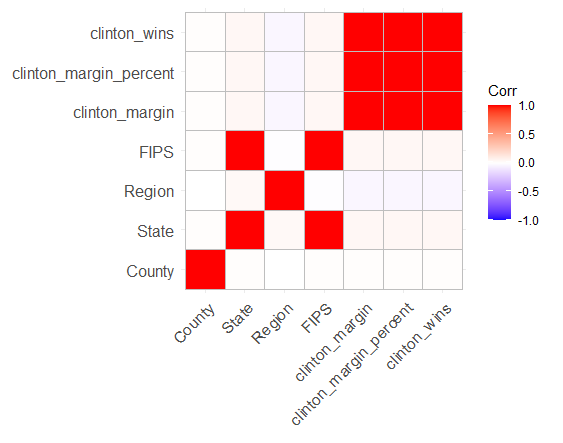
\includegraphics[width=0.90\columnwidth]{assets/cc1.PNG}
    \caption{Correlation Matrix 1 for Clinton}
    \label{lr}
\end{figure}

\begin{figure}[H]
    \centering
    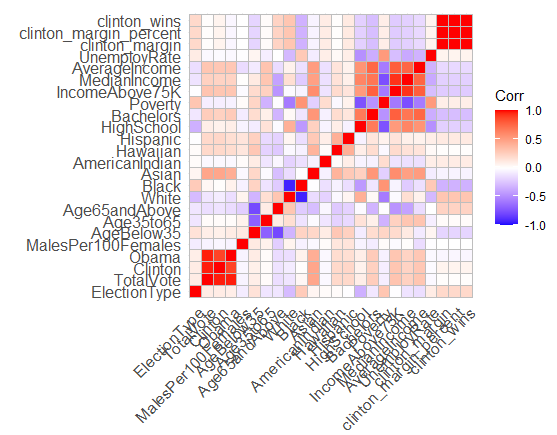
\includegraphics[width=0.90\columnwidth]{assets/cc2.PNG}
    \caption{Correlation Matrix 2 for Clinton}
    \label{lr}
\end{figure}

\begin{figure}[H]
    \centering
    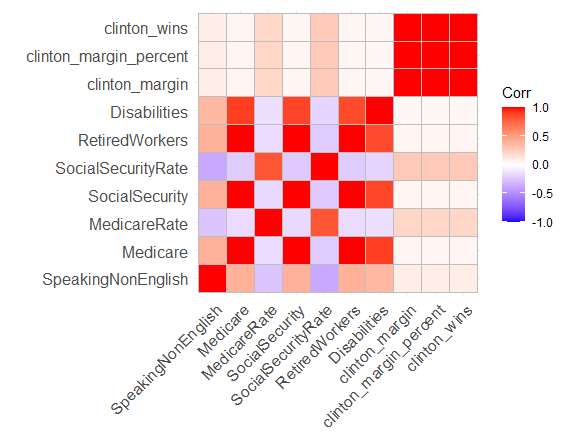
\includegraphics[width=0.90\columnwidth]{assets/cc3.PNG}
    \caption{Correlation Matrix 3 for Clinton}
    \label{lr}
\end{figure}

\begin{figure}[H]
    \centering
    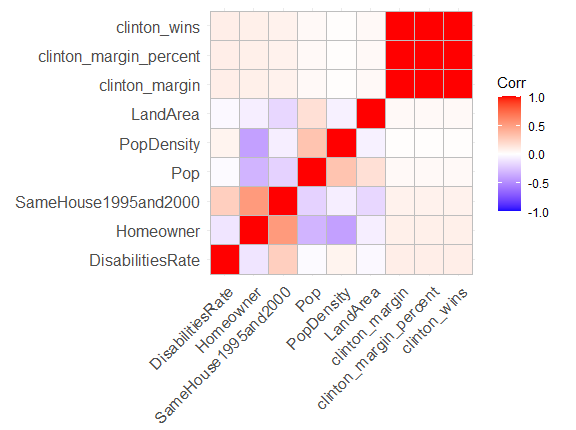
\includegraphics[width=0.90\columnwidth]{assets/cc4.PNG}
    \caption{Correlation Matrix 4 for Clinton}
    \label{lr}
\end{figure}

\subsection{Correlation for Obama}
\subsubsection{R Code for the Correlation Matrices for Obama}
\begin{lstlisting}[language=R]
str(election_data_train)
e<- as.data.frame(election_data_train[,2:5])
a <- as.data.frame(election_data_train[,7:27])
b <- as.data.frame(election_data_train[,43:45])
c <- as.data.frame(election_data_train[,29:35])
d <- as.data.frame(election_data_train[36:42])
election_data_train2 <- cbind(e,b)
election_data_train3 <- cbind(a,b)
election_data_train4 <- cbind(c,b)
election_data_train5 <- cbind(d,b)
vis1 <- (election_data_train2)
library(ggcorrplot)
corr <- cor(vis1)
ggcorrplot(corr)
corr <- as.table(corr)
vis2 <- (election_data_train3)
library(ggcorrplot)
corr <- cor(vis2)
ggcorrplot(corr)
corr <- as.table(corr)
vis3 <- (election_data_train4)
library(ggcorrplot)
corr <- cor(vis3)
ggcorrplot(corr)
corr <- as.table(corr)
vis4 <- (election_data_train5)
library(ggcorrplot)
corr <- cor(vis4)
ggcorrplot(corr)
corr <- as.table(corr)
\end{lstlisting}

\subsubsection{Correlation Matrices for Obama}
\begin{figure}[H]
    \centering
    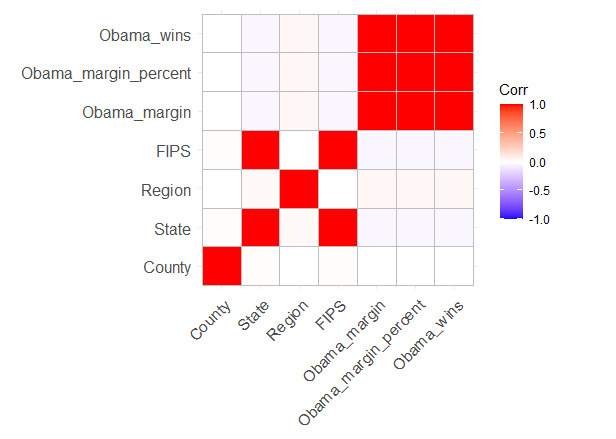
\includegraphics[width=0.90\columnwidth]{assets/oc1.PNG}
    \caption{Correlation Matrix 1 for Obama}
    \label{lr}
\end{figure}

\begin{figure}[H]
    \centering
    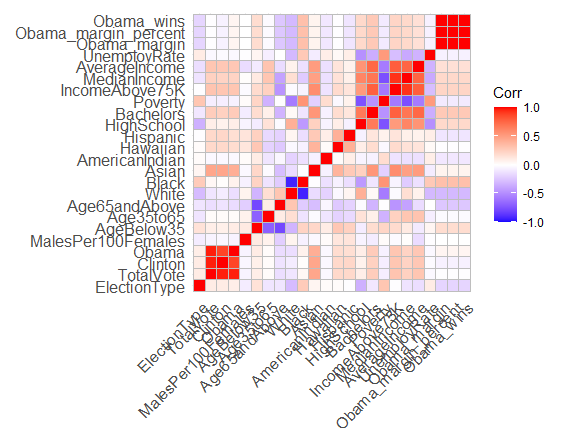
\includegraphics[width=0.90\columnwidth]{assets/oc2.PNG}
    \caption{Correlation Matrix 2 for Obama}
    \label{lr}
\end{figure}

\begin{figure}[H]
    \centering
    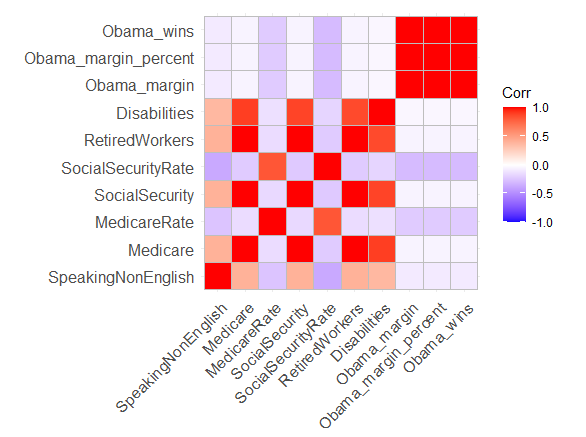
\includegraphics[width=0.90\columnwidth]{assets/oc3.PNG}
    \caption{Correlation Matrix 3 for Obama}
    \label{lr}
\end{figure}

\begin{figure}[H]
    \centering
    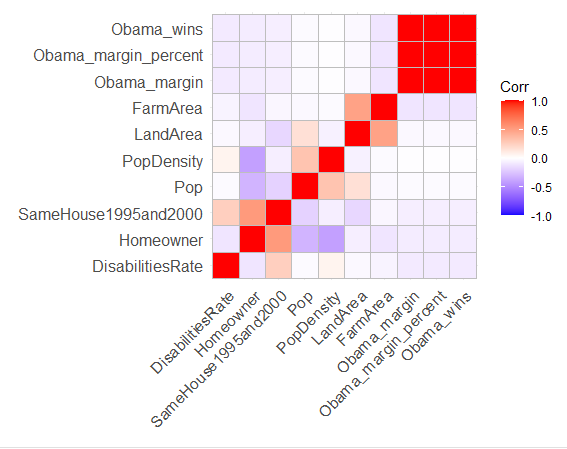
\includegraphics[width=0.90\columnwidth]{assets/oc4.PNG}
    \caption{Correlation Matrix 4 for Obama}
    \label{lr}
\end{figure}




\subsection{Preview of data in Tableau}

\subsubsection{Total votes per candidate}
\begin{figure}[H]
    \centering
    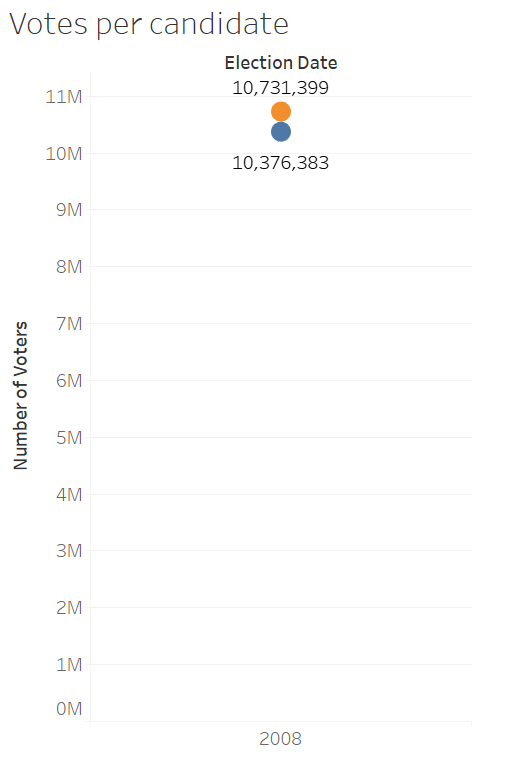
\includegraphics[width=0.90\columnwidth]{assets/vote_candidate.PNG}
    \caption{Votes per candidate }
    \label{lr}
\end{figure}

\subsubsection{Clinton Votes per State}
\begin{figure}[H]
    \centering
    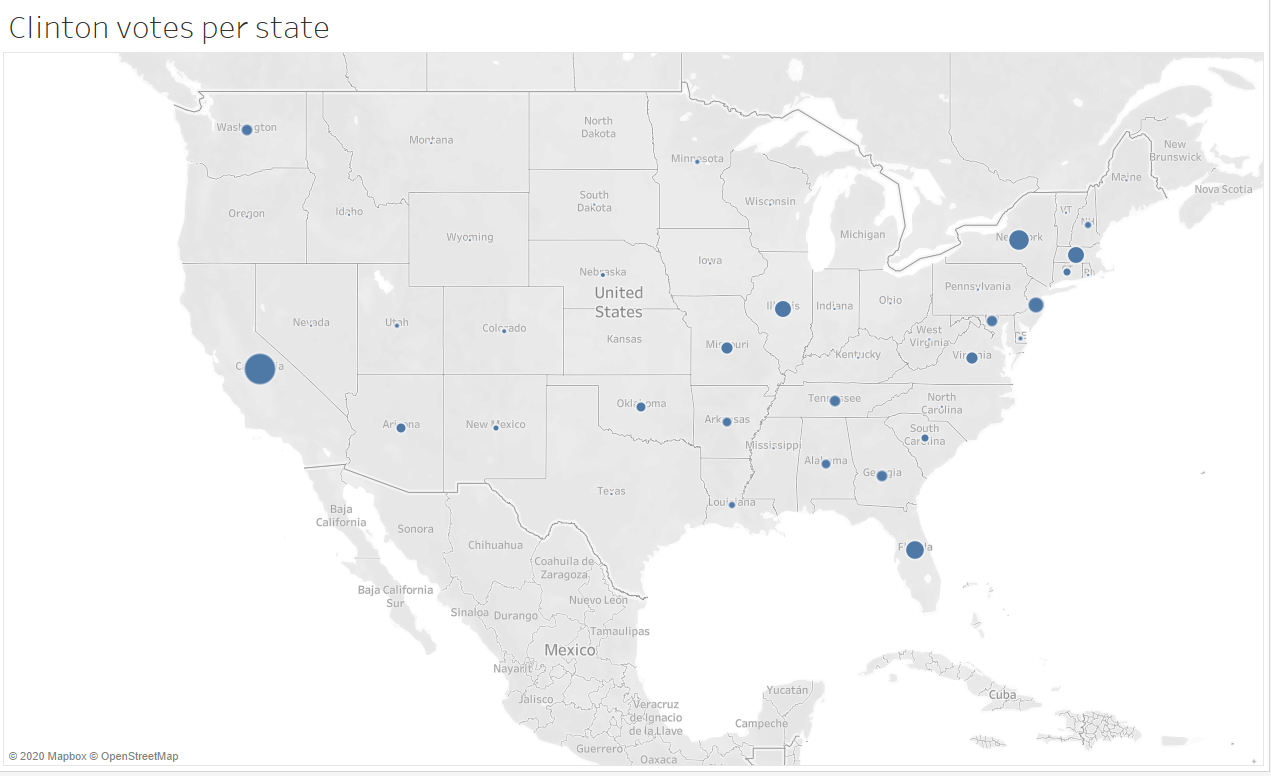
\includegraphics[width=0.90\columnwidth]{assets/clinton_state.PNG}
    \caption{Votes per State on a map of the United States for Clinton }
    \label{lr}
\end{figure}

\subsubsection{Obama votes per State}
\begin{figure}[H]
    \centering
    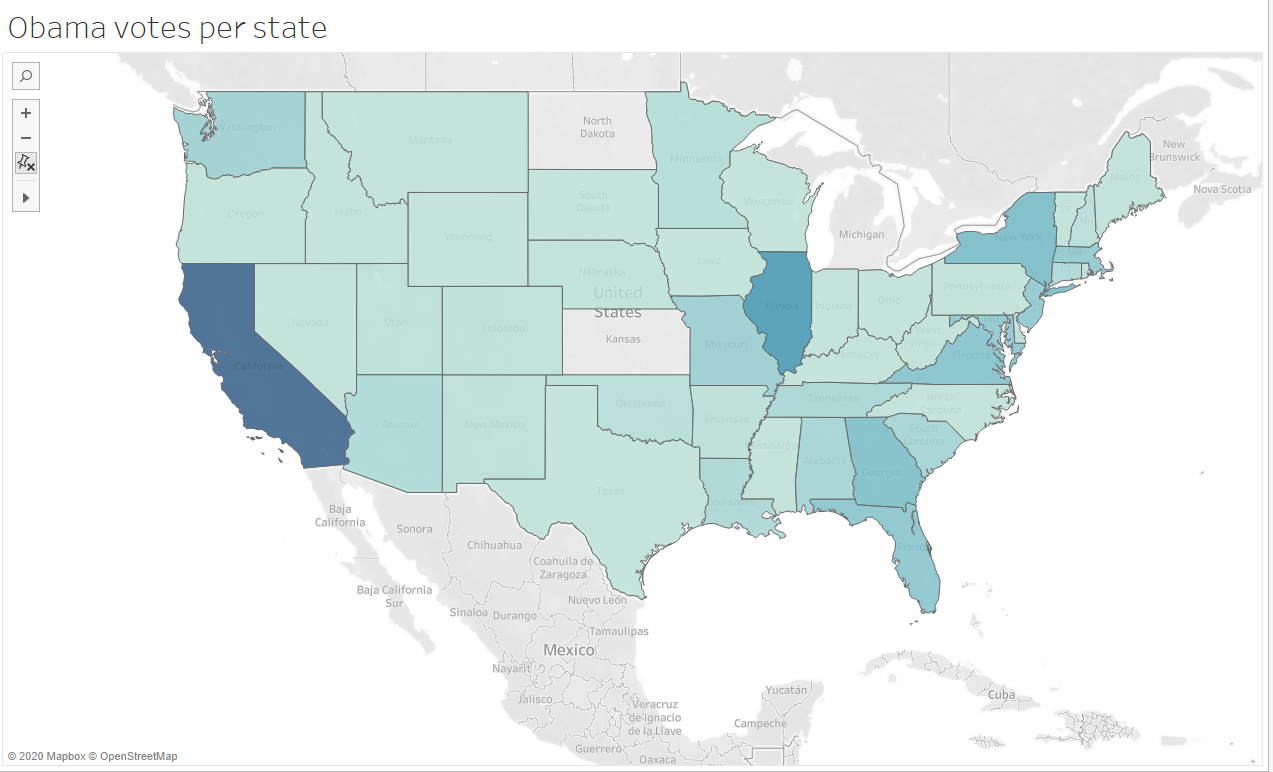
\includegraphics[width=0.90\columnwidth]{assets/obama_state.PNG}
    \caption{Votes per State on a map of the United States for Obama }
    \label{lr}
\end{figure}

\subsubsection{Votes per state and region}
\begin{figure}[H]
    \centering
    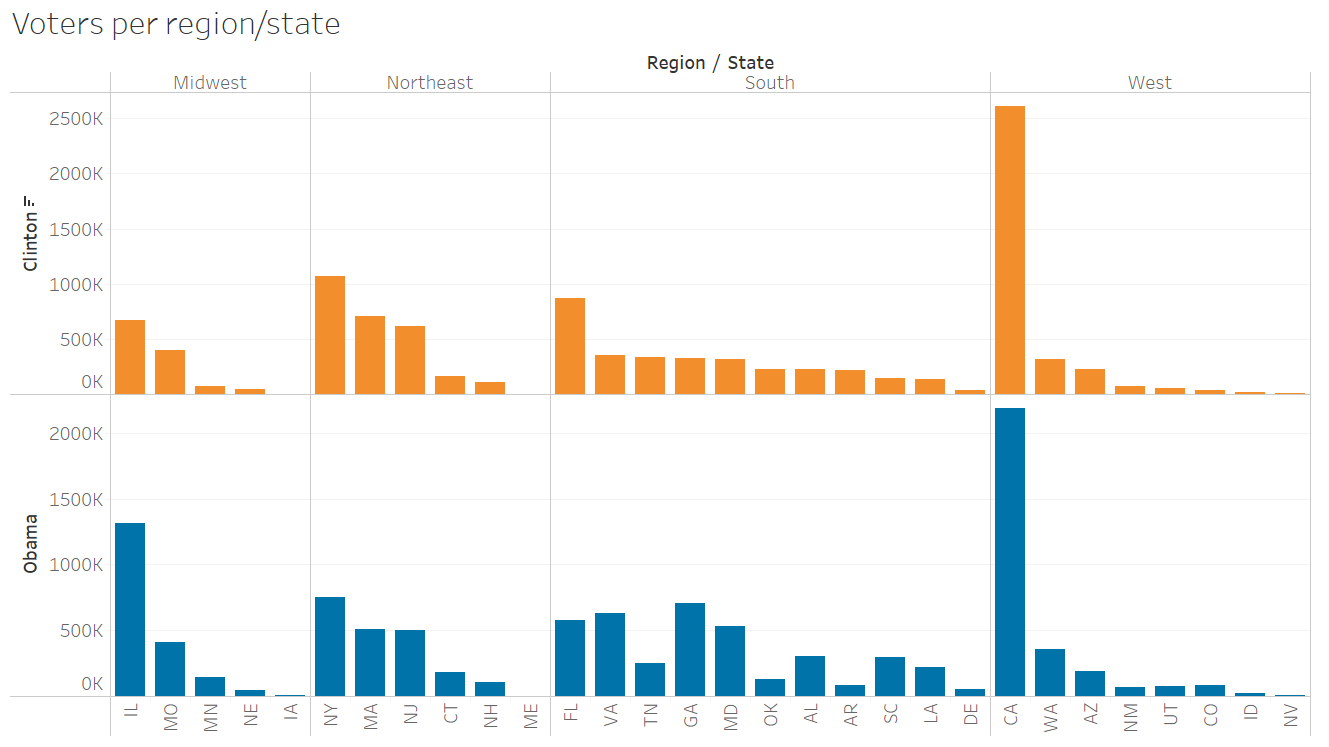
\includegraphics[width=0.90\columnwidth]{assets/vote_region.PNG}
    \caption{Votes per region }
    \label{lr}
\end{figure}

\subsubsection{Votes per month}
\begin{figure}[H]
    \centering
    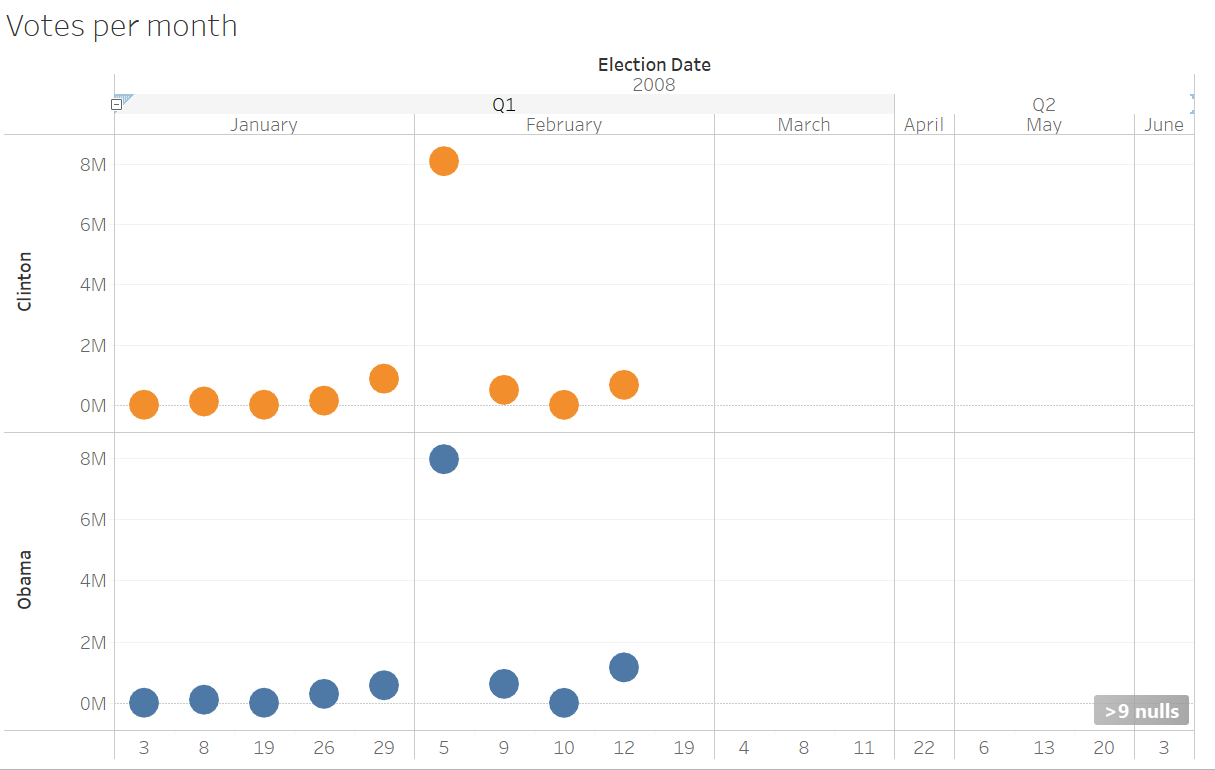
\includegraphics[width=0.90\columnwidth]{assets/vote_month.PNG}
    \caption{Votes per month }
    \label{lr}
\end{figure}

\subsubsection{Votes per age group}
\begin{figure}[H]
    \centering
    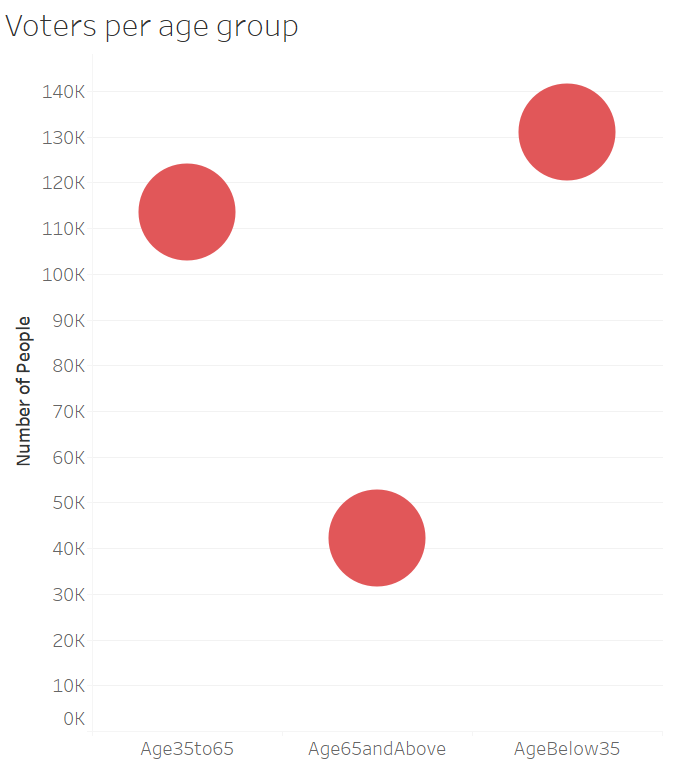
\includegraphics[width=0.90\columnwidth]{assets/vote_age.PNG}
    \caption{Votes per age group }
    \label{lr}
\end{figure}

\subsubsection{Race per region}
\begin{figure}[H]
    \centering
    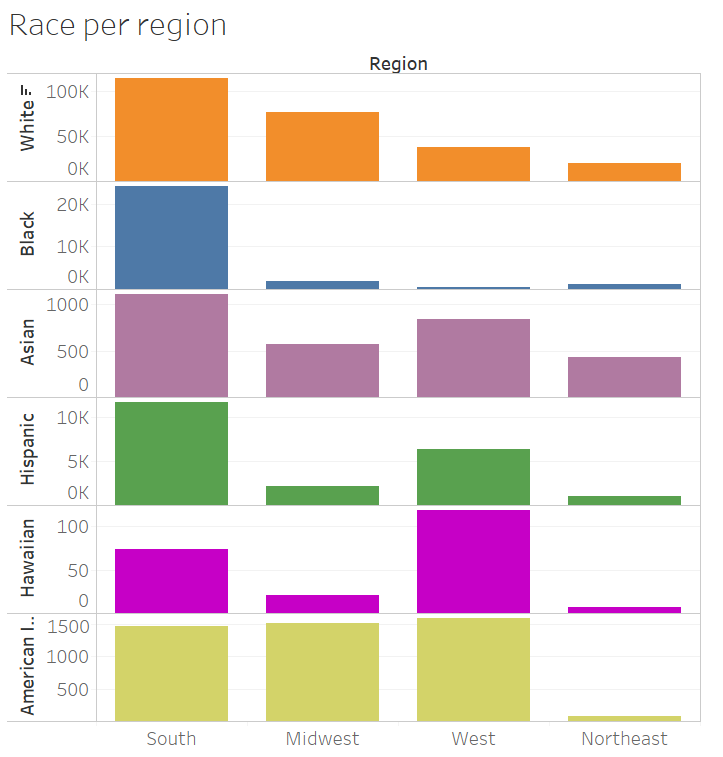
\includegraphics[width=0.90\columnwidth]{assets/race_region.PNG}
    \caption{Distribution of race per region }
    \label{lr}
\end{figure}

\subsubsection{Education per region}
\begin{figure}[H]
    \centering
    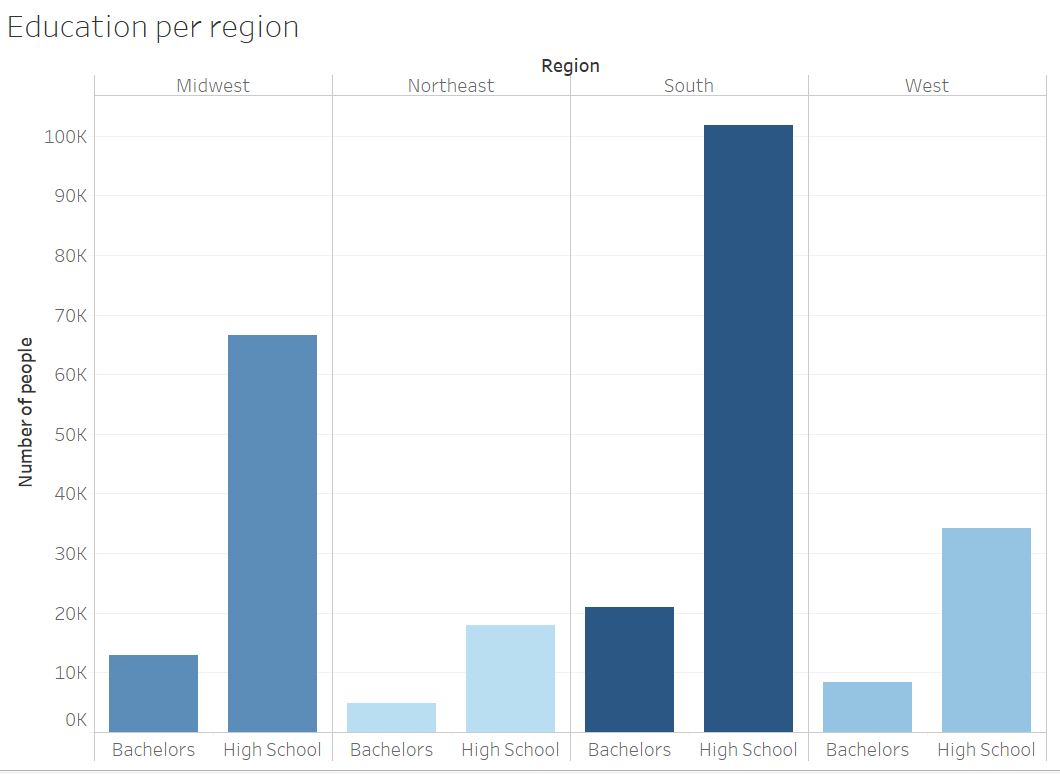
\includegraphics[width=0.90\columnwidth]{assets/education_region.PNG}
    \caption{Distribution of education per region }
    \label{lr}
\end{figure}

\subsubsection{Employment per region}
\begin{figure}[H]
    \centering
    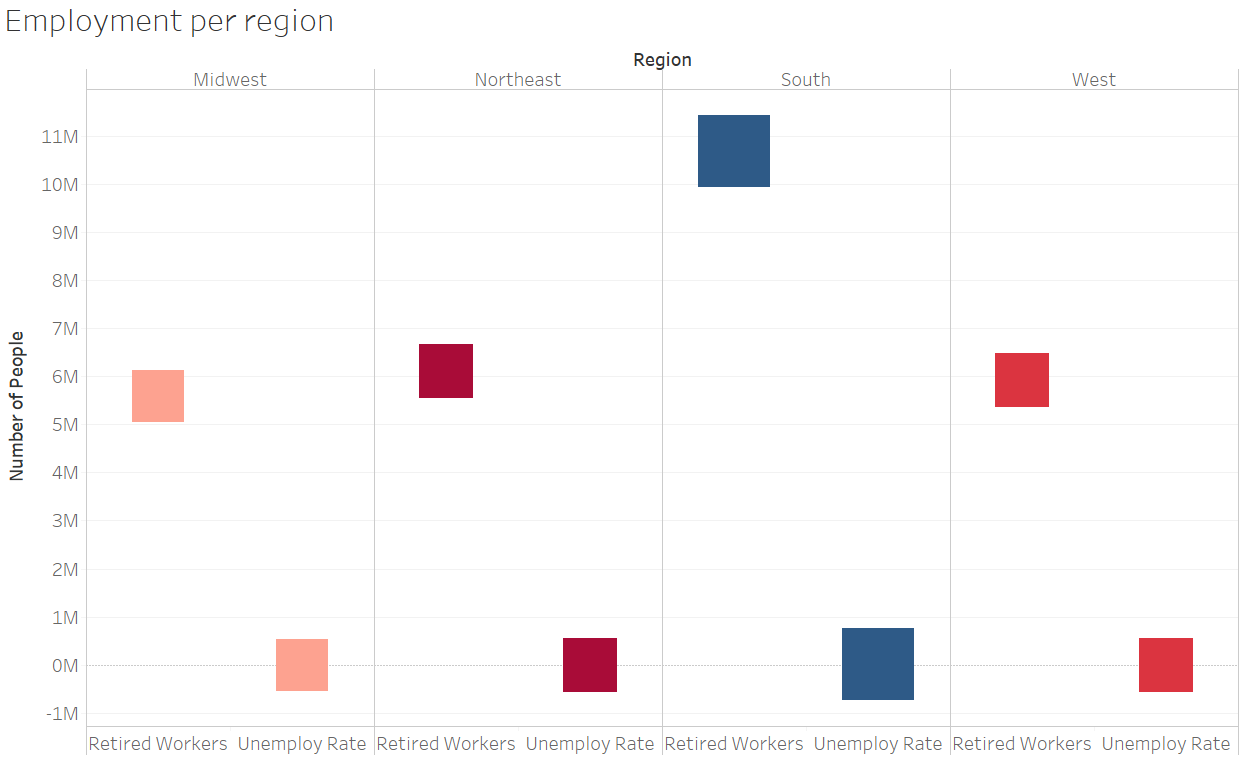
\includegraphics[width=0.90\columnwidth]{assets/employment_region.PNG}
    \caption{Distribution of employment per region }
    \label{lr}
\end{figure}

\subsubsection{Income per region}
\begin{figure}[H]
    \centering
    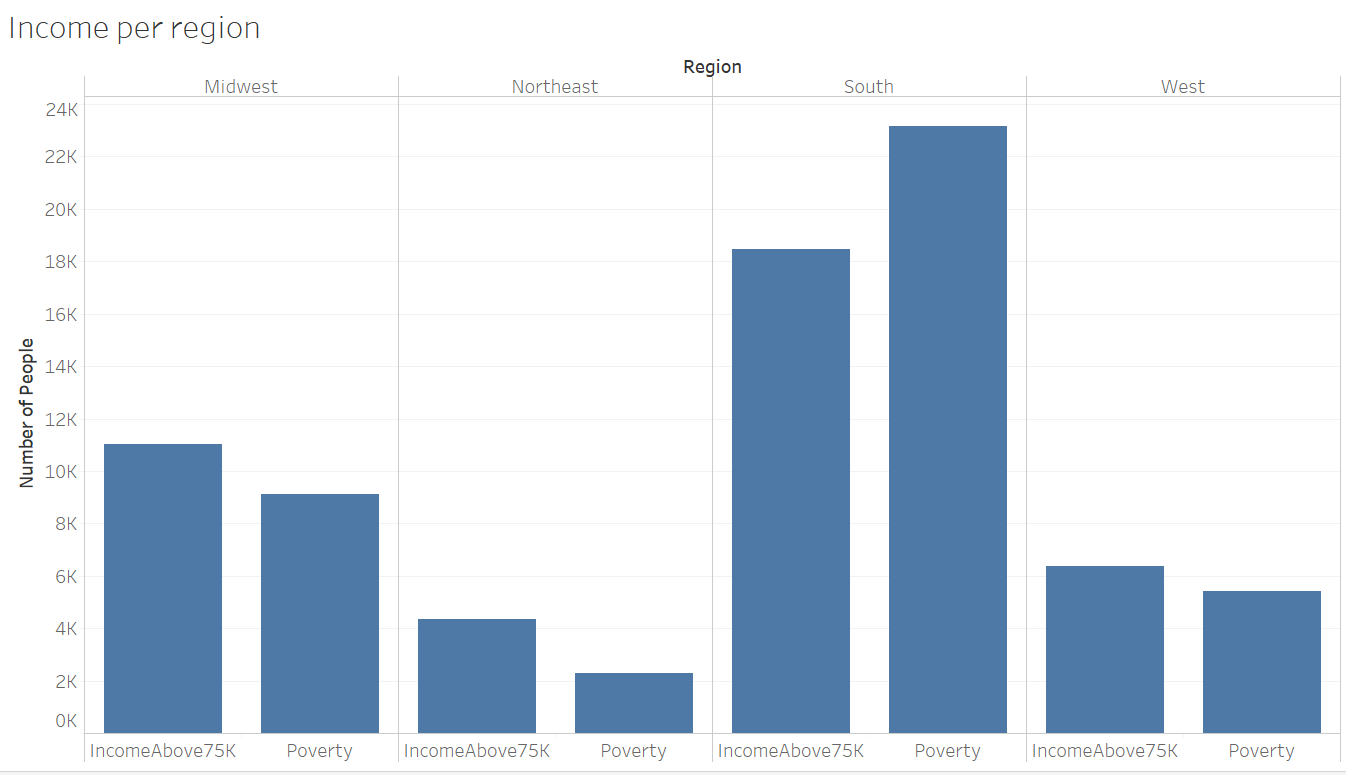
\includegraphics[width=0.90\columnwidth]{assets/income_region.PNG}
    \caption{Distribution of income per region }
    \label{lr}
\end{figure}





\end{document}